%------- 3.1
\subsection{Soma}
    %--- 3.1.1
    \subsubsection{Definição}
        A soma consiste na combinação de 1 ou mais números (parcelas), em um único valor (total). Pode ser representada como uma movimentação pela reta numérica, se estendendo para a direita com números positivos e para a esquerda com números negativos. \eg
        \begin{center}
            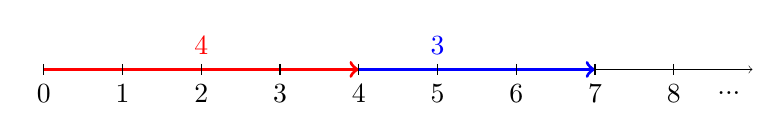
\begin{tikzpicture}
                \draw[black, very thin, ->] (0,0) -- (9,0);
                \node[] at (8.7,-0.3) {...};
                \draw[red, very thick, ->] (0,0) -- (4,0);
                    \node[red] at (2,0.3) {4};
                \draw[blue, very thick, ->] (4,0) -- (7,0);
                \node[blue] at (5,0.3) {3};
                \foreach \x/\xtext in {0/0, 1/1, 2/2, 3/3, 4/4, 5/5, 6/6, 7/7, 8/8} \draw[shift={(\x,0)}] (0pt,2pt) -- (0pt,-2pt) node[below] {$\xtext$};
            \end{tikzpicture}
            \[ 4 + 3 = 7 \]
        \end{center}
    %--- 3.1.2
    \subsubsection{Propriedades}
        \[ a+b = b+a \]
        \[ (a+b)+c = a+(b+c) \]
        \[ a+0=a \]
%------- 3.2
\subsection{Subtração}
    A subtração encontra o valor (diferença) ao reduzir um número (minuendo) por outro (subtraendo). A subtração é a operação inversa da soma, e pode ser reduzida a soma de números de sinais opostos:
    \[ a - b = a + (-b) \]
%------- 3.3
\subsection{Multiplicação}
    %--- 3.3.1
    \subsubsection{Definição}
        A multiplicação produz o resultado (produto) de uma soma finita de números iguais (coeficientes):
        \[ x \cdot y = \underbrace{x + x + ... + x}_\text{y vezes} \]
    %--- 3.3.2
    \subsubsection{Propriedades}
        \begin{multicols}{3}
            \noindent\[ a \cdot b = b \cdot a \]
            \[ (a \cdot b) \cdot c = a \cdot (b \cdot c) \]
            \[ a \cdot (b + c) = ab + ac \]
            \[ a \cdot 1 = a \]
            \[ a \cdot 0 = 0 \]
            \[ 1 \cdot (-1) = (-1) \]
            \[ (-1) \cdot (-1) = 1 \]
            \[ a \cdot \infty = \ ? \]
            \[ (a \cdot b) \in \mathbb{R} \ \forall a,b \in \mathbb{R} \]
        \end{multicols}
%------- 3.4
\subsection{Divisão}
    %--- 3.4.1
    \subsubsection{Definição}
        A divisão é a operação inversa a multiplicação, repartindo um valor (dividendo) em determinado número (quociente) de quantitativos iguais (divisor) através de sucessivas subtrações:
        \[ a \div b = q \ | \ q \cdot b = a \]
    %--- 3.4.2
    \subsubsection{Divisão Inteira}
        Quando limitada ao conjunto dos números inteiros, a divisão pode ser inexata, resultando num coeficiente para o divisor para que seu produto seja o maior número possível sem ultrapassar o dividendo, tendo como diferença o resto:
        \[ a \div b = q, r \ | \ q \cdot b + r = a \]
    %--- 3.4.3
    \subsubsection{Divisibilidade}
        Uma divisão inteira com resto zero estabelece uma relação de divisibilidade, onde o dividendo é dito como divisível pelo divisor. 
    %--- 3.4.4
    \subsubsection{Propriedades}
        \begin{multicols}{2}
            \noindent\[ a \div b \neq b \div a \]
            \[ (a \div b) \div c \neq a \div (b \div c) \]
            \[ (a+b) \div c = a \div c + b \div c \]
            \[ a \div 1 = a \]
            \[ a \div 0 = ? \]
            \[ 1 \div (-1) = (-1) \]
            \[ (-1) \div (-1) = 1 \]
        \end{multicols}
%------- 3.5
\subsection{Módulo}
    Representa o valor absoluto de um número como sua distância até a fonte na reta numérica, independentemente do sentido:
    \[ |a| = |-a| \]
%------- 3.6
\subsection{Números Primos}
    Número primo é todo aquele cujo conjunto dos divisores não inversíveis não é vazio, e todos os seus elementos são produtos dele por números inteiros inversíveis. Resumidamente é todo número inteiro cujo conjunto dos divisores naturais é composto apenas por 1 e ele mesmo.
%------- 3.7
\subsection{Fatoração}
    %--- 3.7.1
    \subsubsection{Definição}
        A fatoração é a decomposição dos coeficientes primos que iteram determinado elemento como seu produto. \eg
        \[ 2520 = 2 \cdot 2 \cdot 2 \cdot 3 \cdot 3 \cdot 5 \cdot 7 \]
    %--- 3.7.2
    \subsubsection{MDC}
        O máximo divisor comum de dois elementos pode ser encontrado ao multiplicar seus fatores primos comuns.
    %--- 3.7.3
    \subsubsection{MMC}
        O mínimo múltiplo comum de dois elementos pode ser encontrado ao dividir o produto desses números pelo seu MDC:
        \[ MMC(a,b) = \frac{a \cdot b}{MDC(a,b)} \]

        Alternativamente, o MMC pode ser encontrado ao fatora-los juntos. 
%------- 3.8
\subsection{Frações}
    %--- 3.8.1
    \subsubsection{Definição}
        É a representação de valores através da razão entre 2 números inteiros. Todo número racional possui infinitas frações equivalentes para representá-lo, que podem ser simplificadas até sua forma irredutível. \eg
        \[ \frac{256}{128} = \frac{64}{32} = \frac{4}{2} = \frac{2}{1} = 2 \]
    %--- 3.8.2
    \subsubsection{Decimais}
        Frações permitem a representação de números decimais e dízimas periódicas através de valores inteiros. \eg
        \begin{multicols}{2}
            \noindent\[ \frac{1}{5} = 0.2 \]
            \[ \frac{1}{3} = 0.\overline{333} \]
        \end{multicols}
    %--- 3.8.3
    \subsubsection{Propriedades}
        \begin{multicols}{3}
            \noindent\[ \frac{a}{c} \pm \frac{b}{c} = \frac{a \pm b}{c} \]
            \[ \frac{a}{c} \cdot \frac{b}{d} = \frac{a \cdot b}{c \cdot d} \]
            \[ \frac{a}{c} \div \frac{b}{d} = \frac{a}{c} \cdot \frac{d}{b} \]
        \end{multicols}
    %--- 3.8.4
    \subsubsection{Utilidades}
        \[ \frac{a}{c} \pm \frac{b}{d} = \frac{^a/_c \cdot MMC(c,d) \pm ^b/_d \cdot MMC(c,d)}{MMC(c,d)} \]
%------- 3.9
\subsection{Exponenciação}
    %--- 3.9.1
    \subsubsection{Definição}
        A exponenciação é definida pela multiplicação de determinado valor (base) por si próprio um determinado número de vezes (expoente). Também pode ser representada como uma função recursiva:
        \begin{multicols}{3}
            [\[ (a \in \mathbb{R}^*),(n \in \mathbb{Z}^*) \]]
            \noindent\[ a^n = a^{n-1} \cdot a \ \forall n \geq 1 \]
            \[ a^0 = 1 \]
            \[ 0^0 = ? \]
            \[ 0^n = 1 \]
            \[ \infty ^ 0 = ? \]
            \[ 1^{\infty} = ? \]
        \end{multicols}
    %--- 3.9.2
    \subsubsection{Propriedades}
        \begin{multicols}{4}
            \noindent\[ a^n \cdot a^m = a^{n+m} \]
            \[ a^n \div a^m = a^{n-m} \]
            \[ (a \cdot b)^n = a^n \cdot b^n \]
            \[ \left(\frac{a}{b} \right)^n = \frac{a^n}{b^n} \]
            \[ (a^n)^m = a^{n \cdot m} \]
            \[ a^{^n/_m} = \sqrt[m]{a^n} \]
            \[ a^{-n} = \frac{1}{a^n} \]
        \end{multicols}
    %--- 3.9.3
    \subsubsection{Utilidades}
        \begin{multicols}{2}
            \noindent\[ a^2 - b^2 = (a+b) \cdot (a-b) \]
            \[ (a \pm b)^2 = a^2 \pm 2ab + b^2 \]
            \newcolumn
            \[ (a \pm b)^3 = a^3 \pm 3a^{2}b + 3ab^2 \pm b^3 \]
            \[ (a+b)^n = \displaystyle\sum_{k=0}^{n} {\binom{n}{k} a^{n-k} b^k} \]
        \end{multicols}
%------- 3.10
\subsection{Radiciação}
    %--- 3.10.1
    \subsubsection{Definição}
        A radiciação é a operação inversa a exponenciação, onde o radicando é igual ao resultado (raiz) elevado a determinado expoente (índice):
        \[ (a \in \mathbb{R}), (n \in \mathbb{Q}^*) \]
        \[ \sqrt[n]{a} = b \ | \ b^n = a \]
    %--- 3.10.2
    \subsubsection{Propriedades}
        \begin{multicols}{3}
            \noindent\[ (\sqrt[n]{a})^m = \sqrt[n]{a^m} \]
            \[ \sqrt[n]{a^m} = \sqrt[n \cdot p]{a^{m \cdot p}} \]
            \[ \sqrt[n]{a \cdot b} = \sqrt[n]{a} \cdot \sqrt[n]{b} \]
            \[ \sqrt[n]{\left(\frac{a}{b} \right)}= \frac{\sqrt[n]{a}}{\sqrt[n]{b}} \]
            \[ \sqrt[n]{\sqrt[m]{a}} = \sqrt[n \cdot m]{a} \]
            \[ \sqrt[n]{a^m} = a^{^m/_n} \]
        \end{multicols}
    %--- 3.10.3
    \subsubsection{Utilidades}
        \begin{multicols}{2}
            \noindent\[ \sqrt{a \pm \sqrt{b}} = \sqrt{\frac{a + \sqrt{a^{2}-b}}{2}} \pm \sqrt{\frac{a - \sqrt{a^{2}-b}}{2}} \]
            \[ \sqrt{a} \approx \frac{a+b}{2 \sqrt{b}} \]
        \end{multicols}
%------- 3.11
\subsection{Logaritmação}
    %--- 3.11.1
    \subsubsection{Definição}
        A logaritmação é uma expressão análoga à exponenciação, onde seu resultado representa o expoente (logaritmo) ao qual um determinado número (base) deve ser elevado para resultar em certo valor (logaritmando):
        \begin{multicols}{2}
            [\[ (a \in \mathbb{R}^{*}-1), (b \in \mathbb{R}^*) \]]
            \noindent\[ \log_{a}b = x \ | \ a^x = b \]
            \[ \operatorname{antilog}_{a}x=b \ | \ \log_{a}b = x \]
            \[ \operatorname{colog}_{a}b = -\log_{a}b \]
            \[ \log b = \log_{10}b \]
            \[ \ln b = \log_{\mathrm{e}}b \]
            \[ \lg b = \log_{2}b \]
        \end{multicols}
    %--- 3.11.2
    \subsubsection{Propriedades}
        \begin{multicols}{2}
            \noindent\[ \log_{a}(b \cdot c) = \log_{a}b + \log_{a}c \]
            \[ \log_{a}(b \div c) = \log_{a}b - \log_{a}c \]
            \newcolumn
            \[ \log_{a}b^{\alpha} = \alpha \log_{a}b \]
            \[ \log_{a}b = \frac{\log_{c}b}{\log_{c}a} = \log_{c}b \cdot \log_{a}c \]
        \end{multicols}
    %--- 3.11.3
    \subsubsection{Utilidades}
        \begin{multicols}{2}
            \noindent\[ \log_{a}b = \frac{1}{\log_{b}a} \]
            \[ \log_{a^{\beta}}b = \frac{1}{\beta}\log_{a}b \]
        \end{multicols}
%------- 3.12
\subsection{Fatorial}
    %--- 3.12.1
    \subsubsection{Definição}
        O fatorial é uma notação para a multiplicação de um número por todos os seus antecessores inteiros:
        \[ (n \in \mathbb{N}^*) \]
        \[ n! = n \cdot (n-1) \cdot ... \cdot 2 \cdot 1 = \displaystyle\prod_{i=0}^{n-1} {n-i}  \]
        \[ 0! = 1! = 1 \]
    %--- 3.12.2
    \subsubsection{Para Números Negativos}
        \[ \Upsilon \pi o \mu o \nu \eta \]
    %--- 3.12.3
    \subsubsection{Utilidades}
        \[ (x+n)! = x! \displaystyle\prod_{k=1}^{n} {x+k} \]
%------- 3.13
\subsection{Coeficiente Binomial}
    %--- 3.13.1
    \subsubsection{Definição}
        É uma notação muito usada em combinatória, matemática diferencial e problemas com funções polinomiais:
        \[ \binom{n}{k} = \frac{n!}{k!(n-k)!} \]
    %--- 3.13.2
    \subsubsection{Relação de Stifel}
        \[ \binom{n}{k} = \binom{n-1}{k-1} + \binom{n-1}{k} \]
%------- 3.14
\subsection{Somatório}
    O somatório é uma notação para uma função recursiva de sucessivas somas:
    \[ \displaystyle\sum_{i=1}^{n} {x_i} = x_1 + x_{2} + ... + x_{n-1} + x_{n} \]
    
    \eg
    \[ \displaystyle\sum_{i=0}^{\infty} {(x!)^{-1}} = \frac{1}{0!} + \frac{1}{1!} + \frac{1}{2!} + ... \]
%------- 3.15
\subsection{Produtório}
    O produtório é uma notação para uma função recursiva de sucessivas multiplicações:
    \[ \displaystyle\prod_{i=1}^{n} {x_i} = x_1 \cdot x_{2} \cdot ... \cdot x_{n-1} \cdot x_{n} \]

    \eg
    \[ \displaystyle\sum_{i=1}^{5} {i} = 1 \cdot 2 \cdot 3 \cdot 4 \cdot 5 \]
%------- 3.16
\subsection{Ordem de Operações}
    Em expressões algébricas, existe uma ordem específica para se efetuar as operações corretamente:
    \[ \verb|parênteses| \prec \verb|expoentes| \prec \verb|multiplicações e divisões| \prec \verb|somas e subtrações| \]